\documentclass[a4paper]{article}
\usepackage[14pt]{extsizes}
%%% Работа с русским языком
\usepackage{cmap}					% поиск в PDF
\usepackage{mathtext} 				% русские буквы в фомулах
\usepackage[T2A]{fontenc}			% кодировка
\usepackage[utf8]{inputenc}			% кодировка исходного текста
\usepackage[english,russian]{babel}	% локализация и переносы

%%% Дополнительная работа с математикой
\usepackage{amsfonts,amssymb,amsthm,mathtools} % AMS
\usepackage{amsmath}
\usepackage{icomma} % "Умная" запятая: $0,2$ --- число, $0, 2$ --- перечисление

%% Номера формул
%\mathtoolsset{showonlyrefs=true} % Показывать номера только у тех формул, на которые есть \eqref{} в тексте.

%% Шрифты
\usepackage{euscript}	 % Шрифт Евклид
\usepackage{mathrsfs} % Красивый матшрифт

%% Свои команды
\DeclareMathOperator{\sgn}{\mathop{sgn}}

%% Перенос знаков в формулах (по Львовскому)
\newcommand*{\hm}[1]{#1\nobreak\discretionary{}
{\hbox{$\mathsurround=0pt #1$}}{}}

%%% Работа с картинками
\usepackage{float}
\usepackage{graphicx}  % Для вставки рисунков
\graphicspath{{pictures/}}  % папки с картинками
\setlength\fboxsep{3pt} % Отступ рамки \fbox{} от рисунка
\setlength\fboxrule{1pt} % Толщина линий рамки \fbox{}
\usepackage{wrapfig} % Обтекание рисунков и таблиц текстом

%%% Работа с таблицами
\usepackage{array,tabularx,tabulary,booktabs} % Дополнительная работа с таблицами
\usepackage{longtable}  % Длинные таблицы
\usepackage{multirow} % Слияние строк в таблице

\usepackage{cite}
\usepackage{csquotes}


%%% Заголовок
\author{Катнов Артем}
\title{Курсовая работа по теме: \\ Моделирование измельчения руды в барабане рудоразмольной мельницы методом дискретных элементов}
\date{\today}

\usepackage[left=3cm,right=1.5cm,top=2cm,bottom=2cm]{geometry}
\linespread{1.5}
%\parindent=1.25cm
%\oddsidemargin=4.6mm
%\textwidth=16cm
%\headheight=0cm
%\headsep=0cm
%\topmargin=-1cm
%\textheight=25.7cm

%\usepackage{caption}
%\usepackage{flafter}
%\usepackage{footmisc}

\usepackage{xcolor}
\usepackage{hyperref}
% цвета для гиперссылок
\definecolor{linkcolor}{HTML}{0000FF} % цвет ссылок
\definecolor{urlcolor}{HTML}{0000FF} % цвет гиперссылок
\hypersetup{linkcolor=linkcolor, urlcolor=urlcolor, colorlinks=true}

\usepackage{cleveref}
%\usepackage{underscore}
%\usepackage{etoolbox}
%\usepackage{lastpage}
%\usepackage{titlesec}
%\usepackage{flafter}
%\usepackage{color}
%\usepackage{mfirstuc}
%\usepackage{nomencl}
%\usepackage{iftex}

\begin{document}

\selectfont
\maketitle
\newpage
\tableofcontents
\newpage

\section{Введение}

\subsection{Введение в метод дискретных элементов}

Впервые метод дискретных элементов (в дальнейшем МДЭ или DEM) был предложен в 1971 году инженерами Cundall P. A. и Otto D. L. Strack \cite{cundall} для моделирования поведения мелких частиц горных пород. 
МДЭ представляет собой совокупность методов для изучения сыпучих сред. 

Сыпучими средами вполне можно назвать любые дискретизированные среды (песок, грунт, зерно и пр.). 
Сыпучая среда сложна в аналитическом представлении, потому что в зависимости от многих факторов она может проявлять твердоподобное, жидкоподобное или комбинированное свойства. 

\begin{figure}[h!]
	\centering
	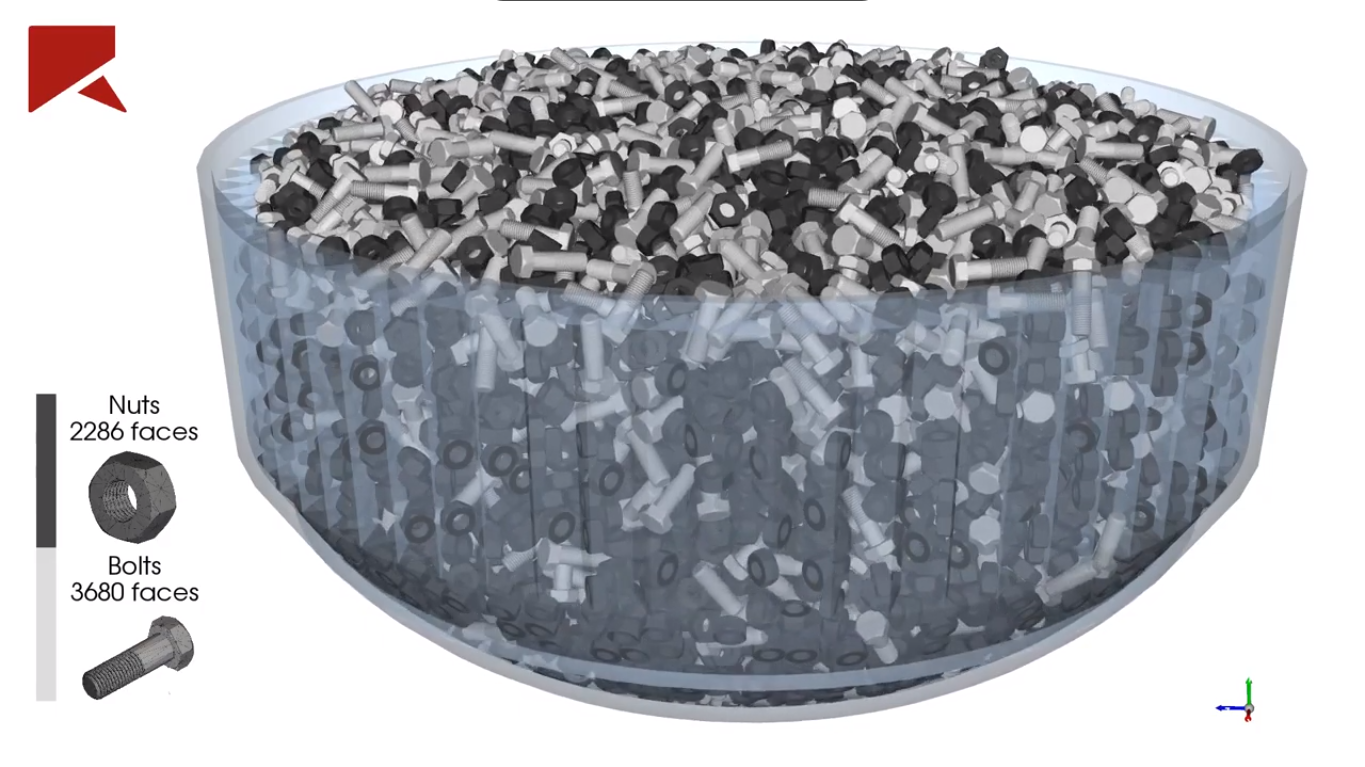
\includegraphics[width=0.5\textwidth]{sreda}
	\caption{Демонстрация сыпучей среды (в данном случае болты и гайки тоже являются сыпучей средой).}
\end{figure} 

Численный расчёт для сыпучих сред проводится независимо для каждого элемента, а взаимодействуют они [элементы] только в точках контакта. 
Основываясь на всем вышесказанном в 1971 году и появился метод дискретных элементов.

Уже на данном этапе мы можем выделить основные преимущество и недостаток данного метода. 
Преимуществом можно назвать возможность моделирования ситуации и сыпучей среды любой сложности без проведения сложных дорогостоящих экспериментов. 
Недостатком же является высокая требовательность к вычислительным ресурсам.

В общем виде работа алгоритма представлена на рисунке \ref{pic:algo}.

\begin{figure}[h!]
	\centering
	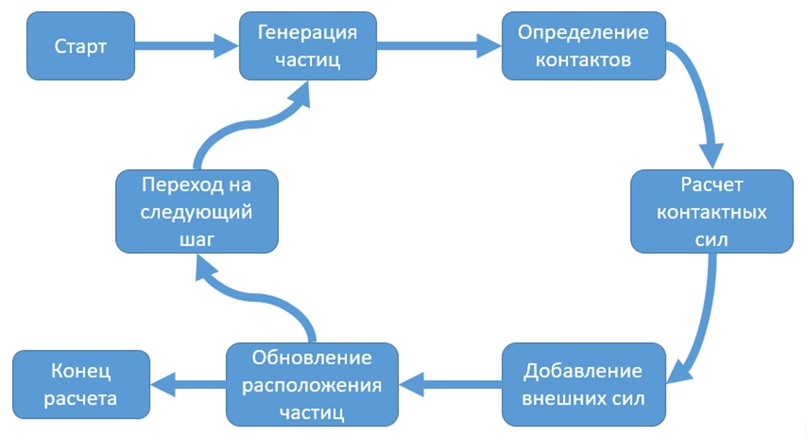
\includegraphics[width=0.7\textwidth]{algorithm}
	\caption{Алгоритм метода в общем виде}
	\label{pic:algo}
\end{figure} 

\subsection{Обзор поставленных задач}

На каждом шаге по времени для найденных взаимодействий происходит расчёт соответствующих контактных сил.
Существует несколько различных моделей силы контакта, подходящих для различных применений, материалов и условий.
Помимо рассмотрения взаимодействия частиц как контактной задачу (с расчётом контактных сил), для анализа положения тел в каждый момент времени применяется так же расчёт скоростей после соударения с использованием закона сохранения импульса.

\begin{figure}[h!]
	\centering
	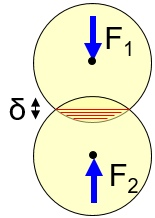
\includegraphics[width=0.2\textwidth]{vhod}
	\caption{Демонстрация контактных сил при пересечении двух шаров.}
\end{figure} 

Силы, действующие на каждую частицу, вычисляются из исходных данных, соответствующих физических законов и выбранной модели контакта (модели контакта необходимо выбирать исходя из условий применения). 
В случае необходимости к расчёту могут быть подключены дополнительные модели: модель когезии, модель демпфирования и т.п., так же хотелось бы отметить что в расчёте могут иметь влияние такие силы, как:

--- Трение, при касании двух частиц

--- Отскакивание, при столкновении

--- Гравитация

--- Притяжение (адгезия, жидкостное соединение)

После определения контактных сил, могут быть добавлены любые другие силы внешнего тела. 
Внешние силы возникают из-за существования одного или нескольких физических полей, таких как гравитационные, электромагнитные или гидродинамические поля.

После нахождения результирующей силы, взаимодействующей на каждую частицу, основываясь на втором законе Ньютона, находится новая позиция всех частиц к началу следующего шага по времени.
Временной шаг сменяется на следующий и цикл повторяется.

Важно также упомянуть, что данный метод не ограничивает расчёт только сферическими телами. Для создания тел любой другой сложной формы можно представить множеством элементов сфер, жёстко связанных между собой (мультисферный агломерат) \cite{aglomerath}.

В данной работе помимо расчёта контактных сил действующих друг на друга также вводятся гравитационное поле, учёт сил трения, а также модель демпфирования. 
В качестве рассматриваемой модели принимается сферическое тело.

\subsection{Обзор аналогов}

Большинство современного программного обеспечения для инженерных расчётов имеет в себе встроенные МДЭ решатели (Ansys Fluent, LS-DYNA), в свою очередь ПО специализирующееся на МДЭ (ESSS Rocky, open-source LIGGGHTS, EDEM (DEM Solutions Ltd.)), зачастую имеет большее широкий спектр возможностей для расчёта поведения сыпучей среды, таких как большее количество моделей контактных сил.

За счёт использования GPU (имеющих большее количество вычислительных ядер), большинство программ преодолело миллион частиц, которые одновременно могут находиться в области расчёта. 
Распараллеливание процессов и введение многопоточной работы может заметно ускорить работу данного итерационного расчёта.

\subsection{Барабанная мельница}
\label{mill_theory}

\begin{figure}[H]
	\centering
	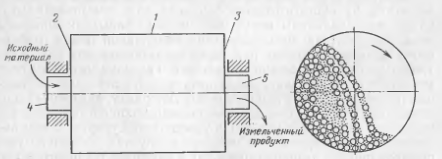
\includegraphics[width=0.6\textwidth]{baraban_shema}
	\caption{Схема барабанной мельницы}
	\label{pic:baraban_shema}
\end{figure} 

Барабанная мельница (рисунок \ref{pic:baraban_shema}) представляет собой пустотелый барабан 1, закрытый торцевыми крышками 2 и 3, в центре которых имеются полые цапфы 4 и 5. 
Цапфы опираются на подшипники и барабан вращается вокруг горизонтальной оси.
Барабан заполняется примерно на половину объема дробящей средой.
При его вращении дробящие тела  благодаря трению увлекаются его внутренней поверхностью, поднимаются на некоторую высоту и свободно или перекатываясь падают вниз.
Через одну полую цапфу внутрь барабана непрерывно подается измельчаемый материал, который проходит вдоль него и, подвергаясь воздействию дробящих тел, измельчается ударом, истиранием и раздавливанием.
Измельченный продукт непрерывно разгружается через другую полую цапфу.


\newpage

\section{Основная часть. Построение математической модели}

\subsection{Упрощения метода дискретных элементов}
В МДЭ есть несколько основных упрощений. 

1) Метод дискретных элементов основан на идее, что выбранный временной шаг настолько мал, что в течение одного временного шага \textbf{возмущения не могут распространяться с любого элемента дальше, чем на его ближайших соседей}. 
Тогда во все времена результирующие силы на любом элементе определяются исключительно его взаимодействием с элементами, с которыми он находится в контакте.
Именно эта ключевая особенность метода отдельных элементов позволяет проследить нелинейное взаимодействие большого числа дисков без чрезмерных требований к памяти.

2) \textbf{Считается, что шары не деформируются.}
Деформации отдельных частиц малы по сравнению с изменением объёма дискретной среды в целом. 
Основная изменение объёма обусловлено прежде всего движением частиц как твёрдых тел. 
Поэтому точное моделирование деформации частиц не является необходимым для получения хорошей аппроксимации механического поведения. 
В данном методе частицам разрешено перекрывать друг друга в точках соприкосновения. 
Это перекрывающее поведение занимает место деформации отдельных частиц. 
Величина перекрытия напрямую связана с контактной силой, как будет описано ниже.
Однако следует отметить, что эти перекрытия малы по отношению к размерам частиц.

Безусловно, задача вычисления индивидуальных траекторий принципиально нелинейна.
Однако, исходя из физических соображений, можно ожидать, что это обстоятельство не повлияет на макроскопическую усреднённую картину процесса.
Тем более что для решения этого вопроса будет проводиться итерационная процедура.

%\subsection{Методику подбора начальных данных}
%(в МДЭ это один из важнейших параметров которому посвящена не одна статья, на данном этапе в нашем случае это итерационный подбор коэффициентов диссипации, шага по времени и поиск зависимости коэффициента жесткости)
%Точность моделирования методом дискретных элементов зависит от начальной плотности, ориентации контакта, размера и формы частиц, а также параметров взаимодействия между частицами, включая контактную жёсткость, коэффициенты трения. 


\subsection{Описание алгоритма}

    
Перейдём непосредственно к описанию работы алгоритма.
В данной работе проводится прямое моделирование процесса во времени.
В первом приближении алгоритм можно представить как схему \ref{pic:algo}. 
Соответственно концом расчёта будем считать состояние равновесия шаров.
Более подробный и точный алгоритм конкретной математической модели на шаге представлен на блок-схеме \ref{pic:osn_block}.

\begin{figure}[h!]
	\centering
	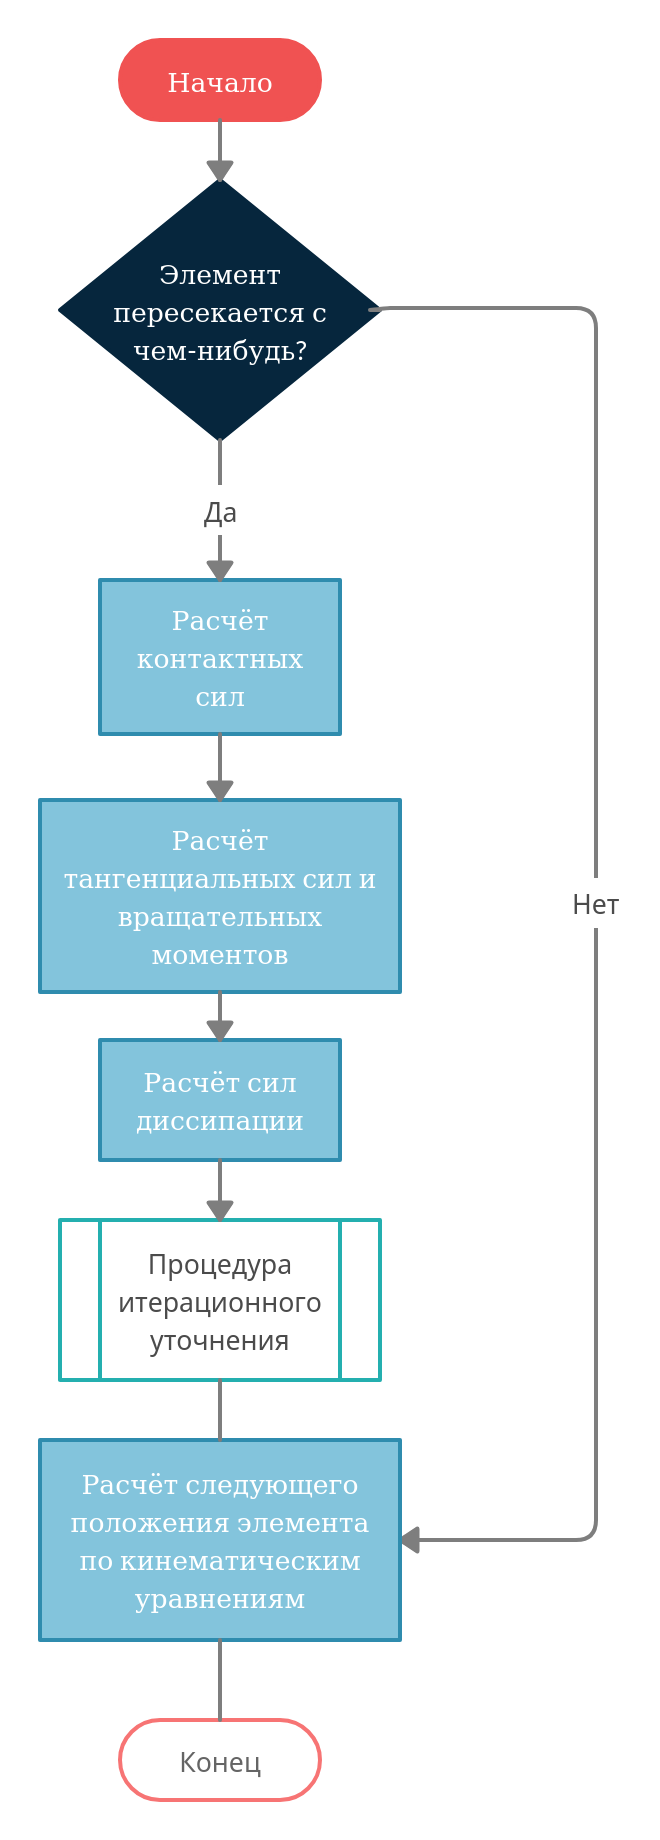
\includegraphics[width=0.4\textwidth]{big_block}
	\caption{Блок-схема работы алгоритма на одном шаге}
	\label{pic:osn_block}
\end{figure} 

В двойном цикле проходимся по каждому возможному сочетанию шаров и проверяем пересекаются ли они.
Если нет -- проверяем следующую возможную пару.
Если да -- необходимо перейти в локальную систему координат, связанную с положением шаров в пространстве друг относительно друга. Все величины, необходимые для расчёта (скорость, ускорение и пр.), переводятся в данную систему координат.

\begin{figure}[h!]
	\centering
	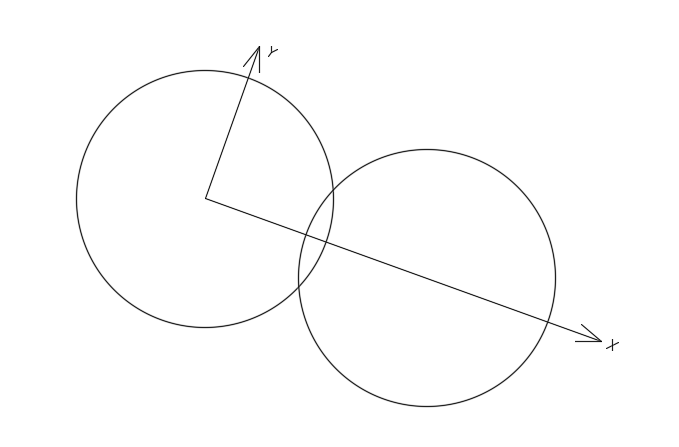
\includegraphics[width=0.4\textwidth]{local}
	\caption{Демонстрация локальной системы координат}
	\label{pic:local}
\end{figure} 

Далее необходимо рассчитать силовые факторы, действующие на шар: силы контактного взаимодействия (по алгоритму \ref{force_subsection}), силы диссипации (по алгоритму \ref{dempf_subsection}), вращательные силовые факторы (по алгоритму \ref{angular_subsection}). 
Нужно также не забыть учесть для каждого из шаров силы удалённого действия которые считаются в каждый момент времени (в нашей модели это будет поле ускорений (пункт \ref{gravitation_subsection})). 
После нахождения сочетания сил действующих на тело проводится итерационную процедуру уточнения (описанную в \ref{iter_subsection})

Когда говорится о каждом возможном сочетании шаров имеется в виду также взаимодействие со стенкой, которой ограничено движение шара. 
В данной работе подробный алгоритм взаимодействия со стенкой описывался в пункте \ref{wall_subsection}.

Итого, второй закон Ньютона при взаимодействии шара с другими объектами имеет следующий вид
\begin{align}
\overline{m \cdot a} &= \overline{F_n} + \overline{F_s} + \overline{D} + \overline{G}\\
\overline{I \cdot \varepsilon} &= \overline{M_s} + \overline{M_r}
\end{align}

где $m$ --- масса элемента, [кг];

$\overline{a}$ --- вектор линейного ускорения элемента от данного взаимодействия, [Н / кг];

$\overline{F_n}$ --- вектор контактной силы, действующий в направлении нормали данного взаимодействия, [Н];

$\overline{F_s}$ --- вектор силы трения скольжения данного взаимодействия, [Н];

$ \overline{D}$ --- вектор сил диссипации, действующих на элемент в результате данного взаимодействия, [Н];

$\overline{G}$ --- вектор сил удалённого действия, действующих на элемент все время, [Н];

$I$ --- момент инерции данного элемента относительно центра, [кг $ \cdot $ м$^2$];

$ \overline{\varepsilon}$ --- вектор углового ускорения элемента от данного взаимодействия, [1 / с$^2$];

$ \overline{M_s}$ --- вектор момента, возникающий в результате перемещения силы трения скольжения в центр (механизм будет показан в следующих пунктах), [Н $ \cdot $ м];

$\overline{M_r}$ --- вектор момента трения качения данного взаимодействия, [Н $ \cdot $ м];
\\

После -- необходим переход в глобальную систему координат.

После расчёта и уточнения всех сил происходит интегрирование -- расчёт нового положения каждого из шаров.

Можем довольно легко оценить сложность этого алгоритма: время -- $O(n^2)$, память $O(n)$. 
Безусловно для большого числа элементов (от 100) такая сложность по времени -- непозволительная роскошь.
Путей решения данной проблемы два.
Первый -- так называемое хэширование. 
Деление пространства на определённые участки и проверка пересечения шаров не со всеми шарами, а только с близлежащими участками.
При правильном выборе сетки, которой покрывается пространство это позволит уменьшить сложность по времени до $O(n)$.

Второй путь решения данной проблемы -- распараллеливание процессов подсчёта на одном шаге разных независимых участков пространство (необходимо сначала будет реализовать первый подход). Это сможет увеличить время подсчёта лишь на константу, но эта константа будет тем больше, чем больше шаров участвует в моделировании.


\subsection{Кинематика частиц}
\label{kinem_subsection}

В данной работе рассматривается элемент с тремя степенями свободы: 2-мя линейными и 1-ой угловой.
В декартовой системе координат они обозначаются как $x$, $y$ и $\vartheta$.
В локальной системе координат эти степени свободы имеют следующие обозначения как $n$, $t$ и $\vartheta$. Соответственно направление нормали к взаимодействию, тангенциальное направление и угловое (не изменяется от перехода от глобальной системы координат к локальной).

Кинематические уравнения для расчёта нового положения тела на шаге могут быть представлены следующим образом
\begin{align}
x &= x_0 + v^x_0 \cdot \Delta t + \dfrac{a^x_0 \cdot \Delta t^2}{2} + \dfrac{b^x_0 \cdot \Delta t^3}{6}\\
y &= y_0 + v^y_0 \cdot \Delta t + \dfrac{a^y_0 \cdot \Delta t^2}{2} + \dfrac{b^y_0 \cdot \Delta t^3}{6}\\
\vartheta &= \vartheta_0 + v^{\vartheta}_0 \cdot \Delta t + \dfrac{a^{\vartheta}_0 \cdot \Delta t^2}{2} + \dfrac{b^{\vartheta}_0 \cdot \Delta t^3}{6}
\end{align}

$b_0^i$ в данных уравнения -- рывок по $i$-той координате. 
Его значение получается в результате итерационного процесса.
Конкретно данная процедура будет обсуждаться в пункте \ref{iter_subsection}.



\subsection{Расчёт контактных сил}
\label{force_subsection}

\textit{Силы в нормальном направлении.}

Контактная сила шаров при их пересечении будет определяться как
\begin{equation}
\label{norm_force}
F_n = k_n \cdot \delta_n
\end{equation}

где $F_n$ --- контактная сила, возникающая в точке контакта и действующая на оба шара, [Н];

$k_n$ --- коэффициент жёсткости, [Н/м];

$\delta_n$ --- взаимное проникновение, так называемое вхождение шаров друг в друга, [м].

При построении модели расчёта сил при взаимодействии элементов друг с другом необходимо определиться с выбором построения модели жёсткости. 
Cundall в своей работе \cite{cundall} описывал постоянную жёсткость, которая зависит исключительно от свойств материала.
\begin{equation}
\label{kn_const}
k_n = const
\end{equation}


Как альтернатива, существует упрощённое решение контактной задачи Герца \cite{friction_calibration}.
Оно используется наиболее часто при моделирование процессов МДЭ.
Исходя из него жёсткость зависит и от свойств материала, и от вхождения, и от радиусов шаров:

\begin{equation}
\label{kn_herz}
k_n = \frac{4}{3} \cdot E_{eff} \cdot \sqrt{R_{eff} \cdot \delta_n}
\end{equation}
где 
\[
\dfrac{1}{E_{eff}} = \dfrac{1 - \nu_1^2}{E_1} + \dfrac{1 - \nu_2^2}{E_2} \qquad \qquad \qquad \dfrac{1}{R_{eff}} = \dfrac{1}{R_1} + \dfrac{1}{R_2}
\]

В дальнейшей работе программы будет выбрана модель Герца.


\textit{Крутящие силовые факторы и силы в тангенциальном направлении}
\label{angular_subsection}


В процессе взаимодействия двух шаров помимо силы в нормальном направлении из-за коэффициентов трения появляются сила в тангенциальном направлении и момент.

\begin{figure}[h!]
	\centering
	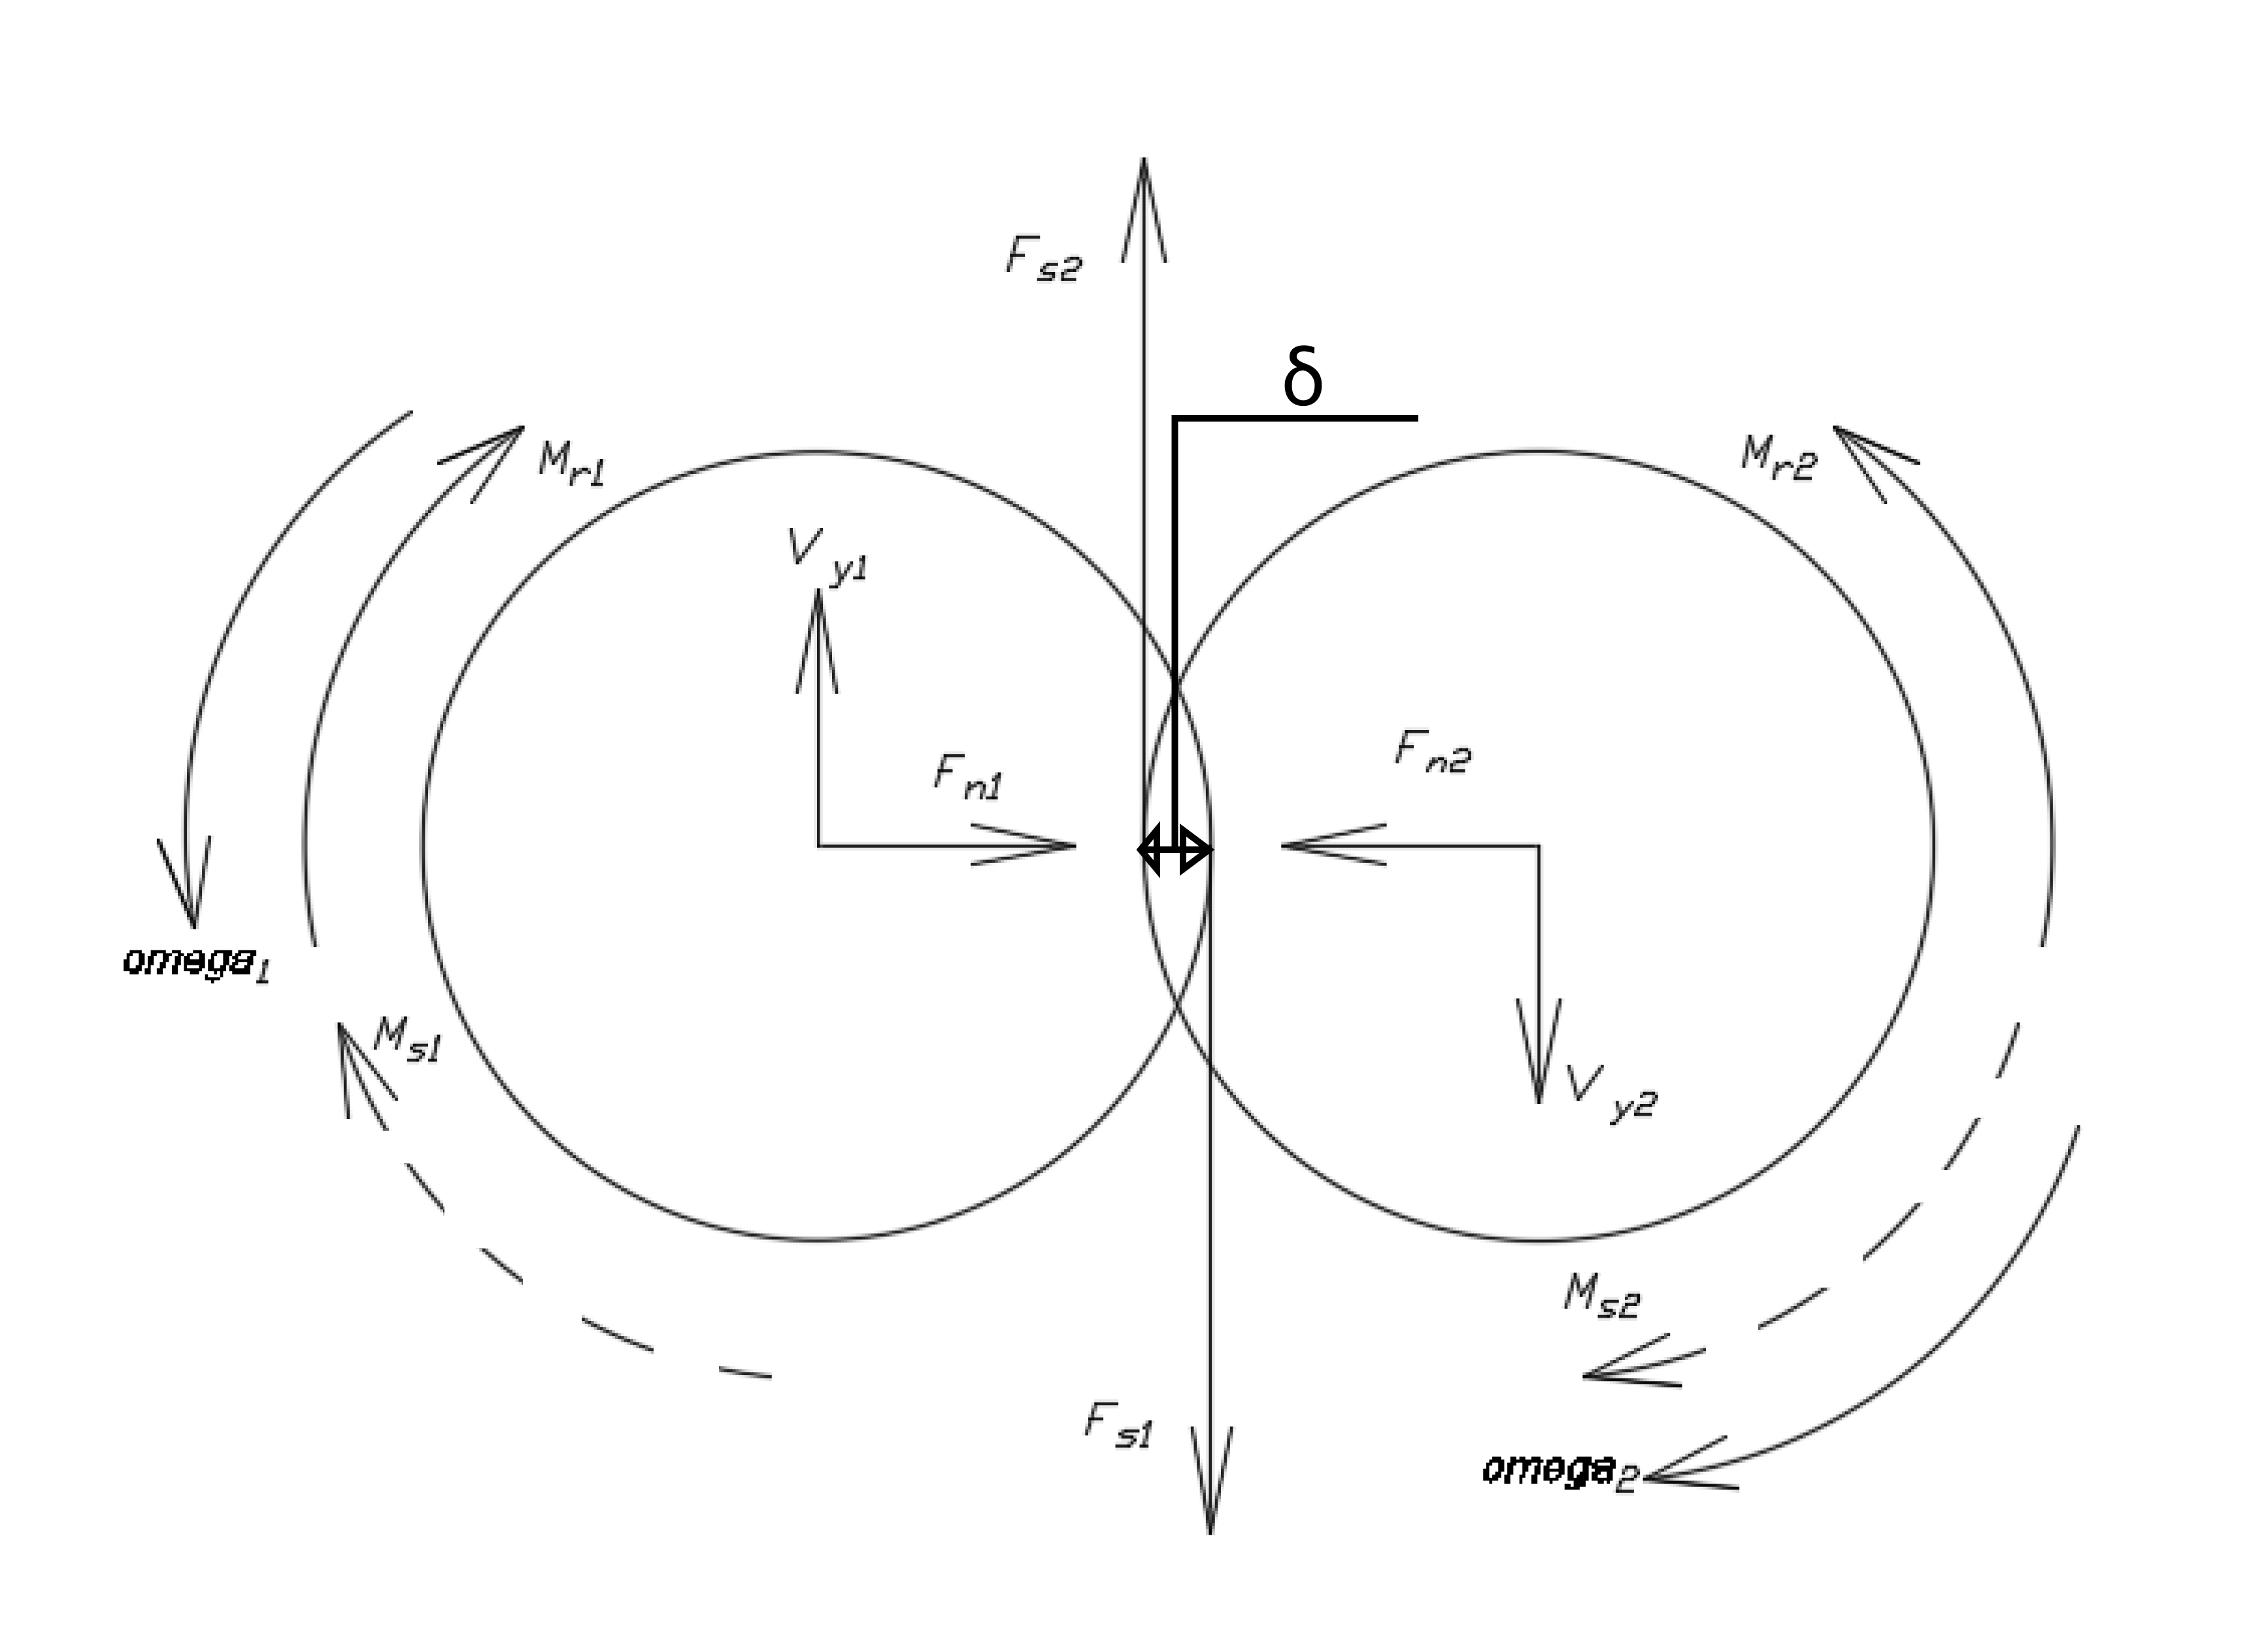
\includegraphics[width=0.8\textwidth]{sily}
	\caption{Силы возникающие в шарах при контактном взаимодействии.}
	\label{pic:sily}
\end{figure} 

Сила в тангенциальном направлении будет появляться из-за трения скольжения и направлена в противоположном относительной тангенциальной скорости шара в точке контакта (относительно другого шара) \cite{friction_calibration}. На рисунке \ref{pic:sily} сила скольжения обозначена $F_s$. Сила скольжения определяется по формуле
\begin{align}
\label{sliding_force}
F_s = \mu_s \cdot F_n \cdot sign(v_{rel\_tan}) \qquad \qquad \qquad v_{rel\_tan} \neq 0
\end{align}

где $\mu_s$ --- безразмерный коэффициент трения скольжения (зависит только от свойств материала);

$F_n$ --- контактная сила действующая на элемент в нормальном направлении, [Н];

$v_{rel\_tan}$ --- тангенциальная скорость шара в точке контакта, относительно другого шара, [м/с].


Отдельного обсуждения стоит расчёт относительной тангенциальной скорости шара. 
Помимо тангенциальной скорости центра шара ($v_y$ на рисунке \ref{pic:sily}) в относительную тангенциальную скорость в точке контакта также будет входить угловая скорость домноженная на радиус шара.
Итого, формула для определения $v_{rel\_tan}$ выглядит следующим образом (верхним индексом обозначены номера шаров: 1 -- шар для которого проводится расчёт, 2 -- шар, вступивший с ним в контакт):
\begin{align}
\label{rel_tan_velocity}
v_{rel\_tan}^{1} = v_{y}^{1} - v_{y}^{2} - \left( \omega_1 \cdot R_1 + \omega_2 \cdot R_2 \right)
\end{align}

\begin{figure}[h!]
	\centering
	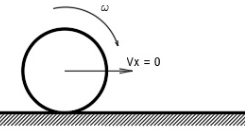
\includegraphics[width=0.4\textwidth]{pol_omega}
	\caption{Шар должен катится по неабсолютно гладкому полу при ненулевой угловой скорости и нулевой линейной.}
	\label{pic:pol_omega}
\end{figure} 

Помимо понятного с точки зрения физического смысла объяснения необходимости учёта добавка угловой скорости можно привести следующий пример. 
Если вращающийся вокруг оси параллельной полу шар (не имеющий линейной скорости) поставить на этот пол, то шар обретёт линейную скорость и покатится (рисунок \ref{pic:pol_omega}). 
Этот эффект объясняется наличием силы трения скольжения и этого самого добавка.

\begin{figure}[h!]
	\centering
	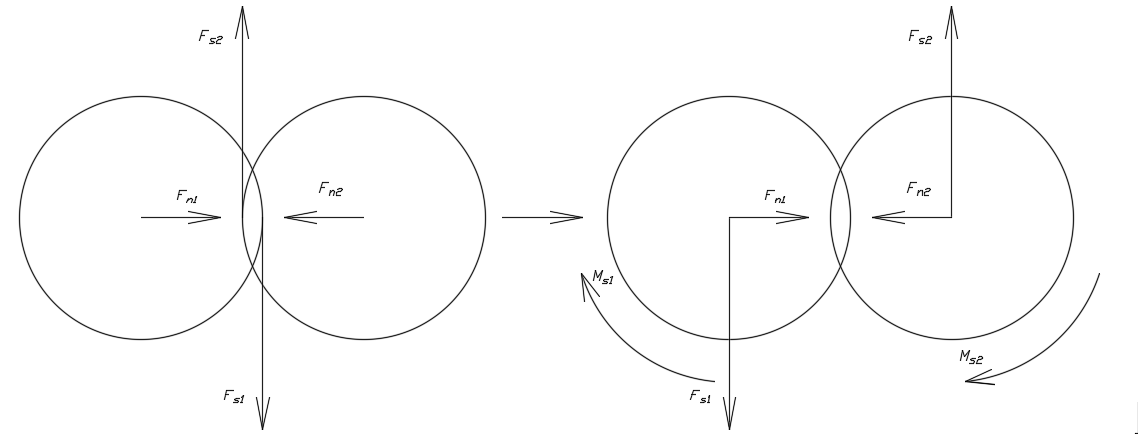
\includegraphics[width=0.8\textwidth]{fs_ms}
	\caption{Приведение силы трения скольжения к центру элемента}
	\label{pic:fs_ms}
\end{figure} 

Из-за того что сила $F_s$ действует в точке контакта при переносе её в центр тяжести от неё появляется момент $M_s$, который определяется по формуле ниже с учётом знака перевода из линейной координаты в угловую (рисунок \ref{pic:fs_ms}).

\begin{align}
\label{sliding_moment}
M_s = F_s \cdot R_{eff}
\end{align}

\[
\text{где} \quad \dfrac{1}{R_{eff}} = \dfrac{1}{R_1} + \dfrac{1}{R_2} \quad \text{ --- эффективный радиус, [м]}
\]

Момент $M_r$ же появляется из-за трения качения и определяется следующим образом.

\begin{align}
\label{rolling_moment}
M_r = \mu_r \cdot F_n \cdot R_{eff} \cdot sign(\omega_{rel}) \qquad \qquad \qquad \omega_{rel} \neq 0
\end{align}

где $\mu_r$ --- безразмерный коэффициент трения качения (зависит только от свойств материала);

$\omega_{rel}$ --- угловая скорость шара, относительно другого шара, [рад/с].

Т.к. $\omega_{rel}$ относительная угловая скорость при внешнем зацеплении шаров она считается по формуле 
\begin{align}
\label{omega_rel}
\omega_{rel} = \omega_1 + \omega_2
\end{align}

В этих формулах вводится эффективный радиус из следующих соображений: если домножать силу на обычный радиус, то на каждом моменте $t$ данного расчёта мы не можем говорить о выполнении второго закона Ньютона (при разных радиусах контактирующих шаров моменты $M_s$ и $M_r$ будут разные по модулю на шарах, участвующих в контакте).
Эффективный радиус же позволяет добиться этого в каждый момент времени.


\subsection{Диссипация}
\label{dempf_subsection}

\begin{figure}[H]
	\centering
	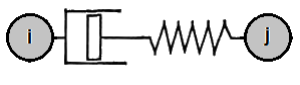
\includegraphics[width=0.4\textwidth]{dempf}
	\caption{При контактном взаимодействии связь шаров можно представить в виде пружины и демпфера.}
	\label{pic:dempf}
\end{figure} 


Силы диссипации возникают, потому что контактное взаимодействие двух шаров воспринимают как пружину с демпфером (рисунок \ref{pic:dempf}). 
Энергия сжатой пружины также будет учитываться далее и записываться как потенциальная.

\[
E_{pot} = \dfrac{k \cdot \delta^2}{2}
\]

где $E_{pot}$ --- энергия сжатия пружины, [Дж];

$k$ --- жёсткость пружины, [Н / м];

$\delta$ --- проникновение шаров друг в друга в направлении нормали, [м].

Силы диссипации линейно зависят от относительной скорости и действуют в противоположном направлении.
Относительная скорость для каждого шара считается в направлении нормали.
Нормалью  далее будем называть направление от центра шара до центра шара с которым он контактирует.
\begin{equation}
\label{dempf_force}
D_n = c_n \cdot v_n
\end{equation}

где $D_n$ --- сила диссипации в нормальном направлении, [Н];

$c_n$ --- коэффициент диссипации в нормальном направлении, [(Н $\cdot$ с) / м];

$v_n$ --- относительная скорость движения шаров в нормальном направлении, [м / с].

Как и силы гравитации в численном методе силы диссипации будут суммироваться и интегрироваться для расчёта положения, скорости и ускорения тела на очередном шаге.

Аналогично, диссипация считается в тангенциальном направлении.
\begin{equation}
\label{dempf_force_tangent}
D_t = c_t \cdot v_t
\end{equation}

где $D_t$ --- сила диссипации в тангенциальном направлении, [Н];

$c_t$ --- коэффициент диссипации в тангенциальном направлении, [(Н $\cdot$ с) / м];

$v_t$ --- относительная скорость движения шаров в тангенциальном направлении, [м / с].

Относительная скорость в нормальном направлении определяется как
\begin{equation}
v_n = v_n^1 - v_n^2
\end{equation}
Относительная скорость в тангенциальном направлении же определяется по формуле \ref{rel_tan_velocity}.

По контактной модели Герца \cite{aglomerath} коэффициенты диссипации непостоянны и зависят не только от обработки элементов и свойств материала, но и от размеров контактирующих шаров и их вхождений друг в друга.
\begin{align}
\label{kef_dempf}
c_n &= 2 \cdot \sqrt{m \cdot 2 \cdot E_{eff} \cdot \delta_n \sqrt{R_{eff}}} \cdot \zeta_n \\
c_t &= 4 \cdot \sqrt{m \cdot 2 \cdot G_{eff} \cdot \delta_n \sqrt{R_{eff}}} \cdot \zeta_t
\end{align}


\subsection{Силы удалённого действия}
\label{gravitation_subsection}

В качестве сил удалённого действия в данной работе выступает только гравитация.
Соответственно
\begin{align}
G^x &= 0 \\
G^y &= m \cdot 9.81
\end{align}

\subsection{Частный случай взаимодействия шар-стена}
\label{wall_subsection}

Элементы в данной модели ограничены стенкой. 
Поэтому необходимо рассмотреть взаимодействие элемент-стена.
Это можно считать частным случаем описанного выше алгоритма с несколькими отличительными чертами.

1) Стенка представлена как замкнутая фигура, состоящая из конечного числа прямых линий.

2) Шар никак не влияет на стенку. 
Её движение зависит только от заданного ей закона движения.

3) При расчёте сил трения используется не эффективный радиус, а радиус данного шара.

4) Стенка вращается относительно какой-то точки.
В данной модели это будет геометрический центр стенки.
Так же важно упомянуть об угловом направлении при вращении стенки.
Если при взаимодействии шаров мы говорили о внешнем зацеплении, то здесь уместно рассматривать внутреннее зацепление шара со стенкой.
Следовательно в формулах \ref{omega_rel} и \ref{rel_tan_velocity} угловая скорость стенки будет идти со знаком минус.


 
\subsection{Итерационное уточнение}
\label{iter_subsection}

%В качестве численного интегрирования в данной работе используется метод прямоугольников (это выходит из принципа 1 упрощений МДЭ).

Интегрирование в данной задаче можно было бы назвать точным, а не численным если бы задача была линейной.
Но данная задача является нелинейной. Если на шаге $t$ на тело действует сила $F_t$, то на следующем шаге $t + \Delta t$ уже будет действовать сила $F_{t + \Delta t}$, которая будет другой и зависеть от величины вхождения шаров друг в друга на момент конца текущего шага по времени, и, следовательно, от закона движения частиц за шаг по времени. 
Закон изменения силы заранее неизвестен.

На первой итерации решения мы принимаем закон изменения сил постоянным (первое приближение к значению силы на конце шага).
Начиная со второй итерации примем изменение силы линейным на шаге от $t$ до $t + \Delta t$  и тогда для интегрирования необходимо ввести ещё один член, который называется рывок. 
Рывок характеризует изменение ускорения.
Обозначим рывок $b_n$.
Тогда
\begin{align*}
a_{t + \Delta t} &= a_t + b_n \cdot \Delta t \\
v_{t + \Delta t} &= v_t + a_t \cdot \Delta t + \dfrac{b_n \cdot \Delta t^2}{2} \\
x_{t + \Delta t} &= x_t + v_t \cdot \Delta t + \dfrac{a_t \cdot \Delta t^2}{2} +  \dfrac{b_n \cdot \Delta t^3}{6}
\end{align*}

Сам по себе рывок можно рассчитать как
\begin{align}
\label{jerk_normal}
b_n = \dfrac{a_{t + \Delta t} - a_{t}}{\Delta t}
\end{align}

Но пока мы не оказались на следующем шаге $a_{t + \Delta t}$ нам не известен.
Поэтому для расчёта рывка проводится итерационный процесс. 
На каждом шаге $t$ проводится расчёт изменения вхождения $\Delta \delta = \delta_{t + \Delta t} - \delta_t$ по следующей формуле
\begin{align*}
\Delta \delta = v_t \cdot \Delta t + \dfrac{a_t \cdot \Delta t^2}{2} +  \dfrac{b_n \cdot \Delta t^3}{6}
\end{align*}

В первую итерацию цикла $b_n$ принимается равным нулю.
Отсюда можем получить перекрытие на следующем шагу $\delta_{t + \Delta t} = \delta_t + \Delta \delta$.
Далее по закону зависимости \ref{norm_force} необходимо найти силу на следующем шаге $F_{t + \Delta t}$ и ускорение $a_{t + \Delta t}$.

Следующим действием нужно проверить удовлетворяет ли нас $a_{t + \Delta t}$ и если нет -- начать итерационную процедуру заново.
Проверкой того что $a_{t + \Delta t}$ нас удовлетворяет и его не надо уточнять (то есть условием выхода из цикла) является критерий выхода из цикла по ускорению.
Это значит, что $a_{t + \Delta t}^k$ должно не значительно отличаться от  $a_{t + \Delta t}^{k-1}$ (верхним индексом отмечен номер итерации на шаге $t$). 
Ещё критерий выхода из цикла можно записать так
\begin{equation}
\label{jerk_condition}
\left| \dfrac{a_{t + \Delta t}^k - a_{t + \Delta t}^{k-1}}{a_{t + \Delta t}^k} \right| < \varepsilon_a
\end{equation}

После нахождения $a_{t + \Delta t}$ по формуле \ref{jerk_normal} можем найти рывок $b$.

Данный процесс показан для нахождения рывка в направлении нормали (понятие нормали было введено в разделе введения  диссипации \ref{dempf_subsection}). 
Процесс нахождения рывков в тангенциальном и угловом направлениях не сильно отличается от указанного выше.

На каждой итерации после нахождения части нормальной контактной силы $\Delta F = F_{t+\Delta t} - F_t$  мы можем найти $\Delta F_s$, $\Delta M_s$, $\Delta M_r$ по формулам \ref{sliding_force}, \ref{sliding_moment} и \ref{rolling_moment}, соответственно.
Аналогично формуле \ref{jerk_normal} находим рывки в тангенциальном и угловом направлениях.
\begin{align}
b_t &= \dfrac{a_{t + \Delta t} - a_{t}}{\Delta t} \label{jerk_tangent}\\
b_{\vartheta} &= \dfrac{\varepsilon_{t + \Delta t} - \varepsilon_{t}}{\Delta t} \label{jerk_angular}
\end{align}

В таком случае условием выхода из цикла будет удовлетворение условию \ref{jerk_condition} для всех трёх направлений одновременно.

Блок-схема данного процесса представлена на рисунке \ref{pic:iter}.

\begin{figure}[H]
	\centering
	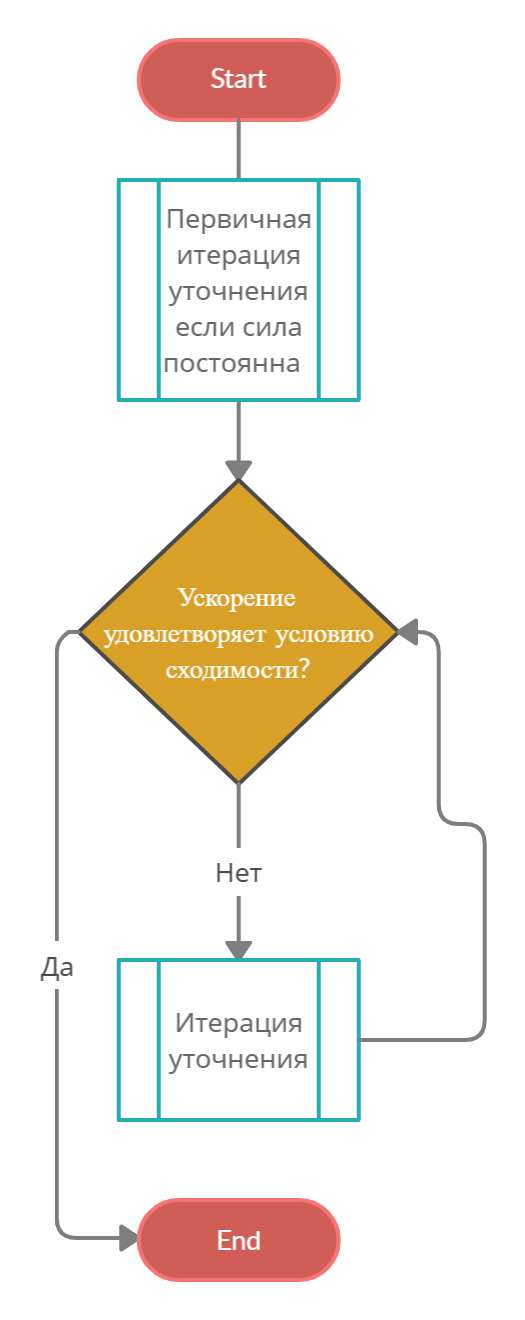
\includegraphics[width=0.4\textwidth]{iter_cicle} 
	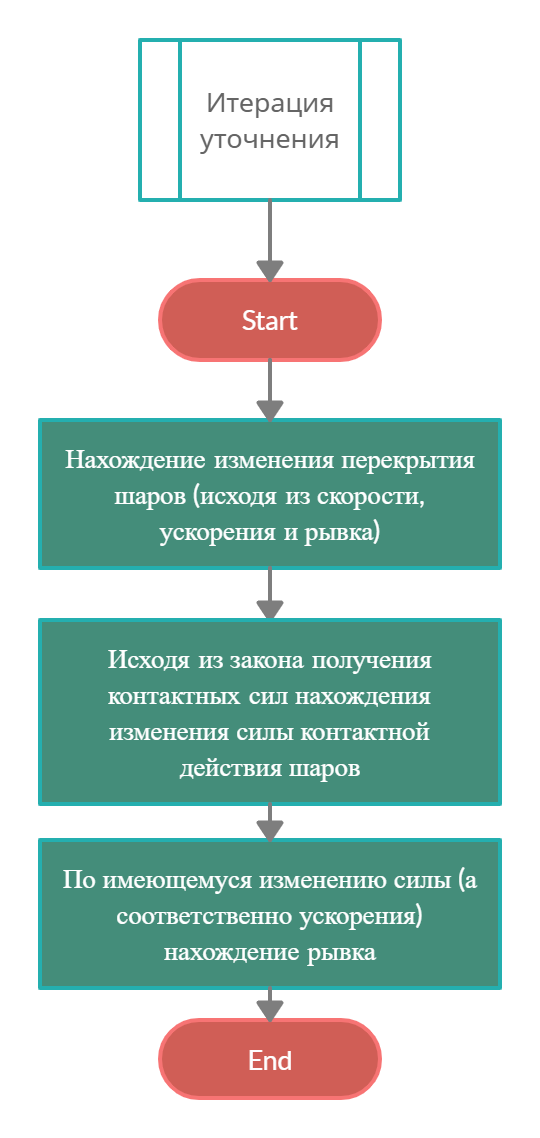
\includegraphics[width=0.4\textwidth]{iter_one}
	\caption{Блок-схема итерационного процесса: слева цикл и условие выхода, справа -- сама процедура уточнения (одна итерация)}
	\label{pic:iter}
\end{figure} 


\subsection{Анализ и проверка адекватности существующей модели}

В качестве проверки адекватности построения данной модели, а также проверки ошибок в решении были использованы несколько различных подходов.

1) Для проверки физичности и логичности результатов использовалось отображение положения и движения шаров.
При прорисовке, например, каждого сотого или тысячного кадра это не так заметно сказывалось на скорости работы программы (время одной прорисовки мало по сравнению с расчётом ста шагов N-го количества шаров), но позволяло оценить корректность и найти логические ошибки на самых ранних стадиях построения решения.

2) Для проверки энергетической составляющей работы алгоритма (а также для корректности диссипирующей модели) использовались графики изменения энергии всей системы во времени (при нулевой диссипации энергия должна быть неизменной, при ненулевой -- энергия должна падать, а система приходить к состоянию равновесия) (рисунок \ref{pic:graphs}) и графики изменения скорости и контактной силы (рисунок \ref{pic:graphs}). Нижепрведенные графики являются примером и не могут быть проанализированы вне контекста.


\begin{figure}[h!]
	\centering
	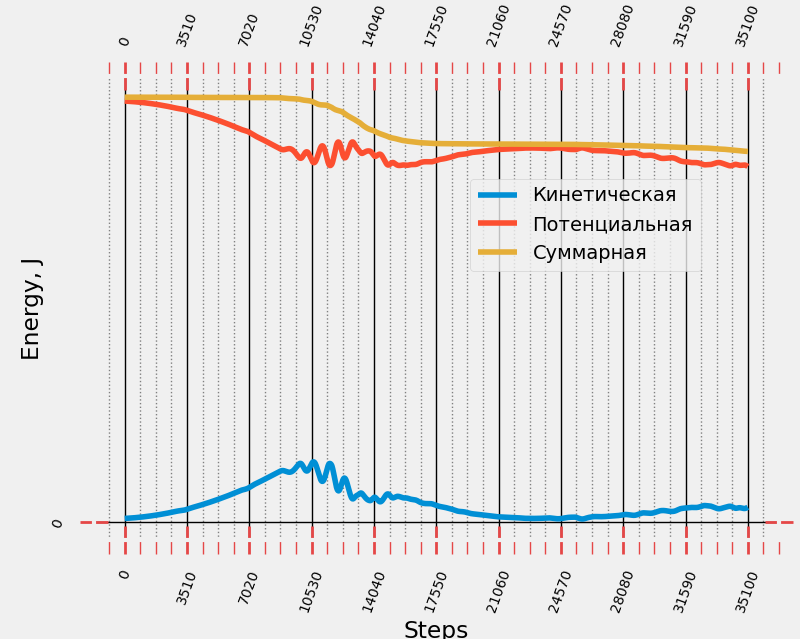
\includegraphics[width=0.4\textwidth , height=0.25\textheight]{graph1} 
	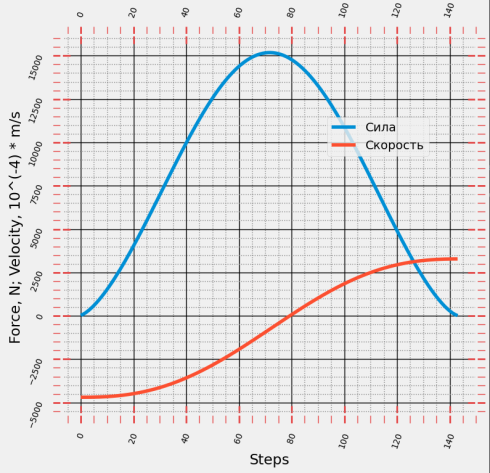
\includegraphics[width=0.4\textwidth , height=0.25\textheight]{graph2}
	\caption{Графики зависимости энергии, силы и скорости}
	\label{pic:graphs}
\end{figure} 

3) Для проверки корректности вращательных модели был проведён ряд тривиальных тестов (около 20 штук) каждый из которых можно было посчитать руками. 
Проверялись корректность направления возникающих сил, моментов и скоростей при различных ситуациях (два шара с нулевой линейной скоростью и ненулевой угловой контактируют, два шара с нулевой угловой скоростью и ненулевой линейной контактируют и пр.) (рисунок \ref{pic:test_primer})
Каждый из этих тестов был пройден.

\begin{figure}[h!]
	\centering
	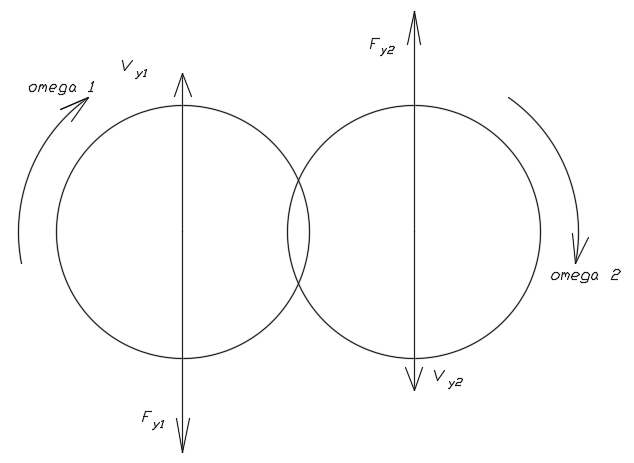
\includegraphics[width=0.4\textwidth]{test_primer} 
	\caption{Пример теста: известны скорости шаров: можем проанализировать направления сил и угловой скорости}
	\label{pic:test_primer}
\end{figure} 

\newpage

\section{Постановка задачи}

\subsection{Механика дробящей среды шаровой мельницы}

Устройство барабанной мельницы довольно подробно представлено в пункте \ref{mill_theory}.
Шаровой называется барабанная мельница в которой в качестве дробящего материала используются стальные или чугунные шары.

Режим работы шаровой мельницы определяется частотой вращения барабана.
При низкой частоте вращения мельницы шары непрерывно цикрулируют, поднимаясь по концентрическим круговым траекториям и скатываясь параллельными слоями каскадом вниз.
Такой режим работы мельницы называется каскадным.

\begin{figure}[H]
	\centering
	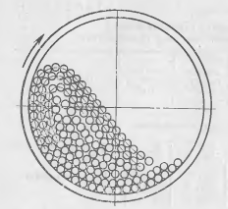
\includegraphics[width=0.3\textwidth]{kaskad_theory} 
	\caption{Схема шаровой нагрузки при каскадном режиме работы мельницы}
	\label{pic:kaskad_theory}
\end{figure} 

По мере повышения частоты вращения мельницы шары по круговым траекториям поднимаются все выше но режим работы может оставаться каскадным.
Когда, наконец, шары поднимутся до известной, еще большей высоты, определяемой частотой вращения мельницы, они сойдут с круговых траекторий и, как тела, брошенные под углом к горизонту, будут падать по параболическим траекториям водопадом обратно на круговые траектории.
Такой режим работы называется водопадным.

\begin{figure}[H]
	\centering
	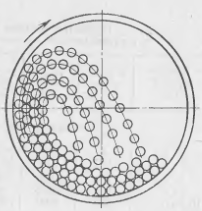
\includegraphics[width=0.3\textwidth]{vodopad_theory} 
	\caption{Схема шаровой нагрузки при водопадном режиме работы мельницы}
	\label{pic:vodopad_theory}
\end{figure} 

Резкого перехода от чисто каскадного режима к чисто водопадному режиму не наблюдается.
Переход происходит постепенно и при промежуточных частотах вращения мельница работает при смешанном каскадно-водопадном режиме.
При таком режиме внешние слои шаров будут падать по параболическим траекториям, но не на свои круговые, а на внутренние слои, скатывающиеся по склону вниз согласно каскадному режиму.

\begin{figure}[H]
	\centering
	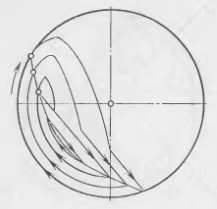
\includegraphics[width=0.3\textwidth]{smeshan_theory} 
	\caption{Схема шаровой нагрузки при смешанном каскадно-водопадном режиме работы мельницы}
	\label{pic:smeshan_theory}
\end{figure} 

Для того чтобы шар поднялся по круговой траектории до наивысшей точки, частота вращения барабана должна вызвать центробежную силу инерции, равную или превосходящую силу тяжести.
При дальнейшем движении после наивысшей точки шар с круговой траектории не сойдет или, как говорят, будет центрифигурировать.

Формула для критической частоты выражается следующим образом

\begin{equation}
\label{freq_kritic}
n_0 = \dfrac{1}{\sqrt[4]{1 - \varphi}} \cdot \dfrac{30 \cdot \sqrt{g}}{\pi \cdot \sqrt{R}}
\end{equation}
где $n_0$ --- частота вращения мельницы, [оборотов в минуту];

$\varphi$ --- отношение объёма, занятого шарами к внутреннему объёму мельницы;

$R$ --- радиус мельницы, [м].

\begin{figure}[H]
	\centering
	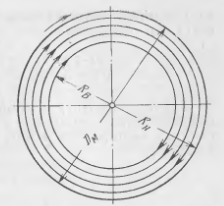
\includegraphics[width=0.3\textwidth]{kritic_theory} 
	\caption{Схема шаровой нагрузки при при превышении критической частоты}
	\label{pic:kritic_theory}
\end{figure} 

\subsection{Реальные параметры}

Для моделирования данной задачи рассматривалась только дробящая среда (без руды). 
В качестве дробящих элементов использовались стальные шары радиусом 20 см.
Коэффициенты трения и скольжения приняты следующим образом
\[
\mu_s = 0.1 \qquad \qquad \qquad \mu_r = 0.05
\]
Коэффициенты диссипации в нормальном и тангенциальном направлениях
\[
\zeta_n = 0.1 \qquad \qquad \qquad \zeta_t = 0.1
\]
Стенка тоже принята стальной и имеет все те же параметры.
Мельница имеет радиус 2.5 м.
В мельницы будет находиться 120 шаров.
Это значит, что по объему она заполнена на 21 \%.

Таким образом можем определить $n_0$ по формуле \ref{freq_kritic}. 
В нашем случае $n_0 = 20$ оборотов в минуту (или 2.1 рад / с).

Шаг по времени равен 10$^{-5}$ секунды.
Каждый эксперимент  проводился в течение 10 секунд.
В реальности расчёт конечно занимал больше времени.
\newpage

\section{Результаты моделирования}

В качестве результатов рассмотрим моделирование работы шаровой мельницы при различных режимах и сравним полученное с ожидаемым.

\subsection{Каскадный режим работы}

При частоте вращения мельницы 0.2 рад / с (1.9 оборотов в минуту) можем наблюдать каскадный режим работы.
Графики изменения энергии (этот и следующие: \ref{pic:kaskad_energy}, \ref{pic:vodopad_energy}, \ref{pic:smeshan_energy}, \ref{pic:kritic_energy}) показывает, что диссипирующая система, которая получает постоянную подпитку энергией извне (стенка крутится, тем самым разгоняя шары) приходит к примерно равновесному по энергии состоянию.

\begin{figure}[H]
	\centering
	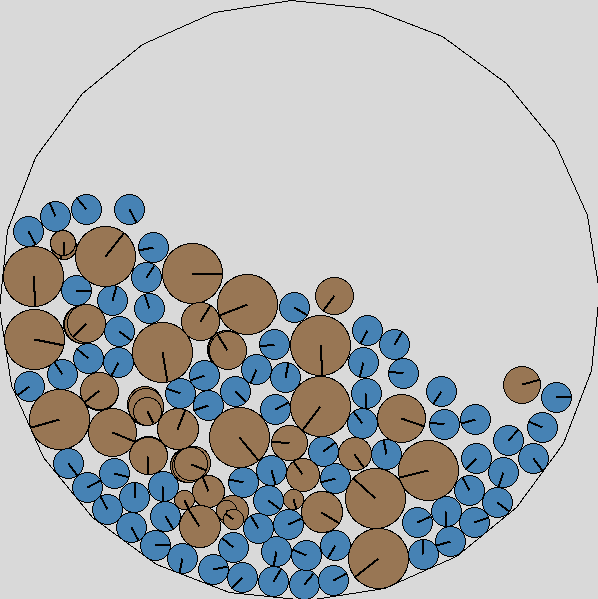
\includegraphics[width=0.5\textwidth]{kaskad_result} 
	\caption{Экспериментальная схема шаровой нагрузки при каскадном режиме работы мельницы}
	\label{pic:kaskad_result}
\end{figure} 

\begin{figure}[H]
	\centering
	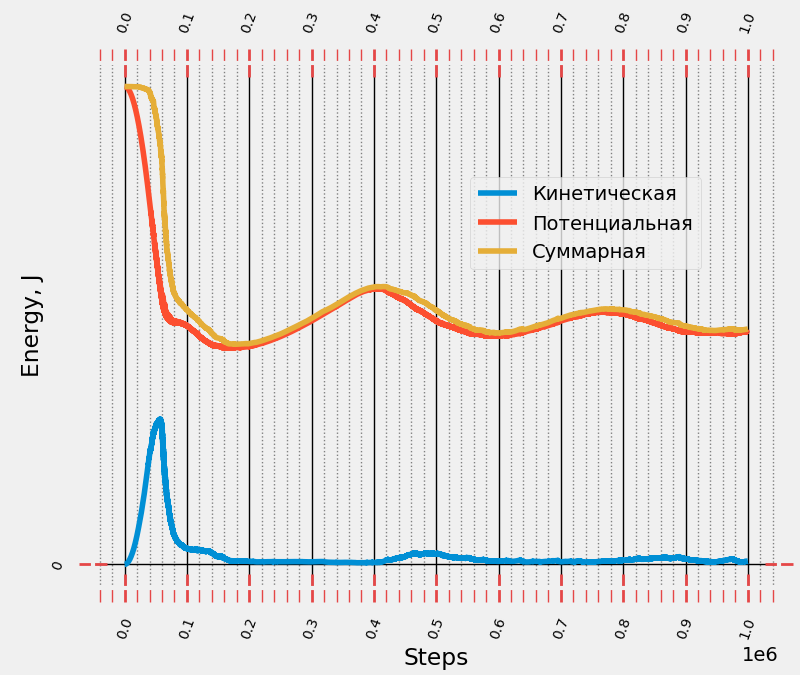
\includegraphics[width=0.5\textwidth]{kaskad_energy}
	\caption{График изменения энергии во времени при каскадном режиме работы мельницы}
	\label{pic:kaskad_energy}
\end{figure} 

\subsection{Водопадный режим работы}

Данный режим работы достигается при 1.8 рад / с (17.19 оборотов в минуту).
Для более выразительной картины данного режима (рисунок \ref{pic:vodopad_theory}) количество шаров увеличено до 240. 
Таким образом заполненность мельницы увеличивается до 42 процентов что близко к максимальному кпд. 

\begin{figure}[H]
	\centering
	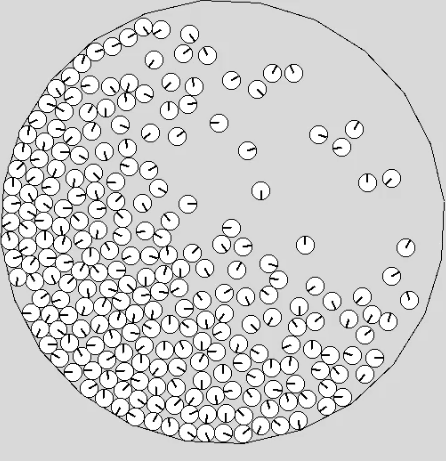
\includegraphics[width=0.5\textwidth]{vodopad_result} 
	\caption{Экспериментальная схема шаровой нагрузки при водопадном режиме работы мельницы}
	\label{pic:vodopad_result}
\end{figure} 

\begin{figure}[H]
	\centering
	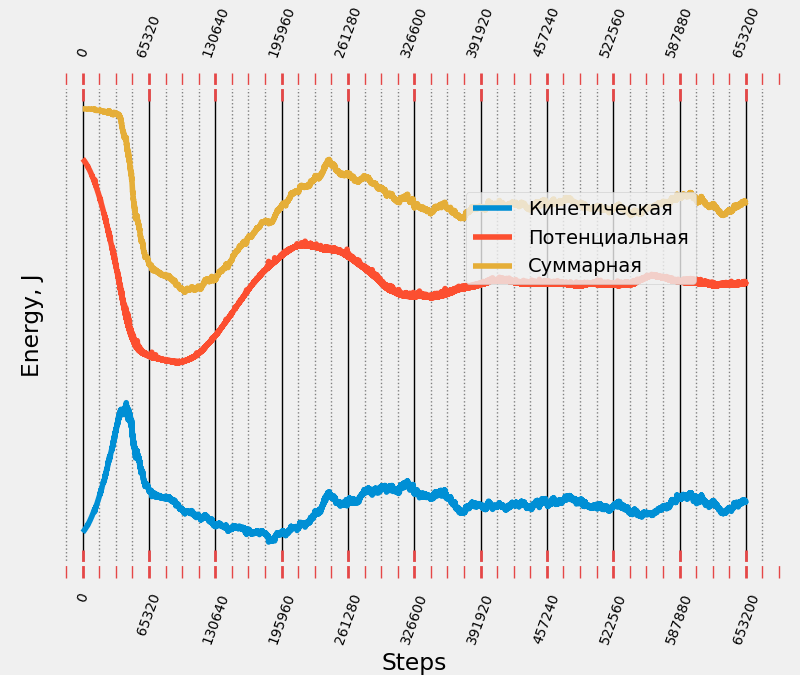
\includegraphics[width=0.5\textwidth]{vodopad_energy} 
	\caption{График изменения энергии во времени при водопадном режиме работы мельницы}
	\label{pic:vodopad_energy}
\end{figure} 

\subsection{Смешанный каскадно-водопадный режим работы}

Данный режим работы достигается при 1.5 рад / с (14.32 оборотов в минуту).

\begin{figure}[H]
	\centering
	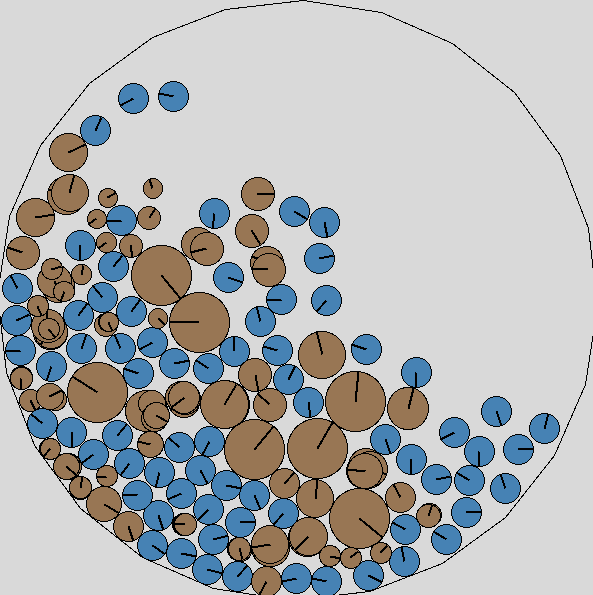
\includegraphics[width=0.5\textwidth]{smeshan_result} 
	\caption{Экспериментальная схема шаровой нагрузки при смешанном каскадно-водопадном режиме работы мельницы}
	\label{pic:smeshan_result}
\end{figure} 

\begin{figure}[H]
	\centering
	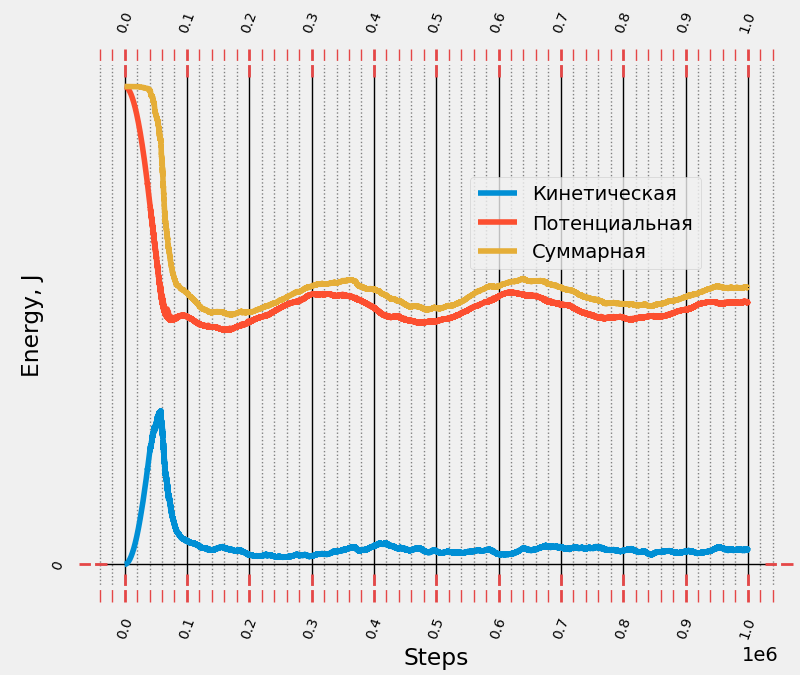
\includegraphics[width=0.5\textwidth]{smeshan_energy} 
	\caption{График изменения энергии во времени при смешанном каскадно-водопадном режиме работы мельницы}
	\label{pic:smeshan_energy}
\end{figure} 

\subsection{Режим работы мельницы при закритической частоте}

Для более быстрого установления характерной картины (рисунок \ref{pic:kritic_theory}) выберем частоту работы мельницы, превышаюшую теоретическую в несколько раз.
В данном примере мельница врашается со скоростью 10 рад / с (95.49 оборотов в минуту).

\begin{figure}[H]
	\centering
	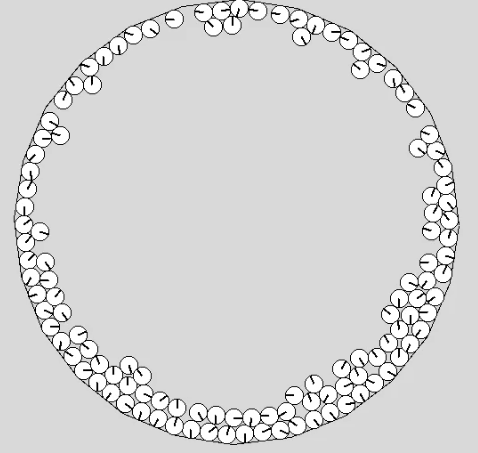
\includegraphics[width=0.5\textwidth]{kritic_result} 
	\caption{Экспериментальная схема шаровой нагрузки при при превышении критической частоты}
	\label{pic:kritic_result}
\end{figure} 

\begin{figure}[H]
	\centering
	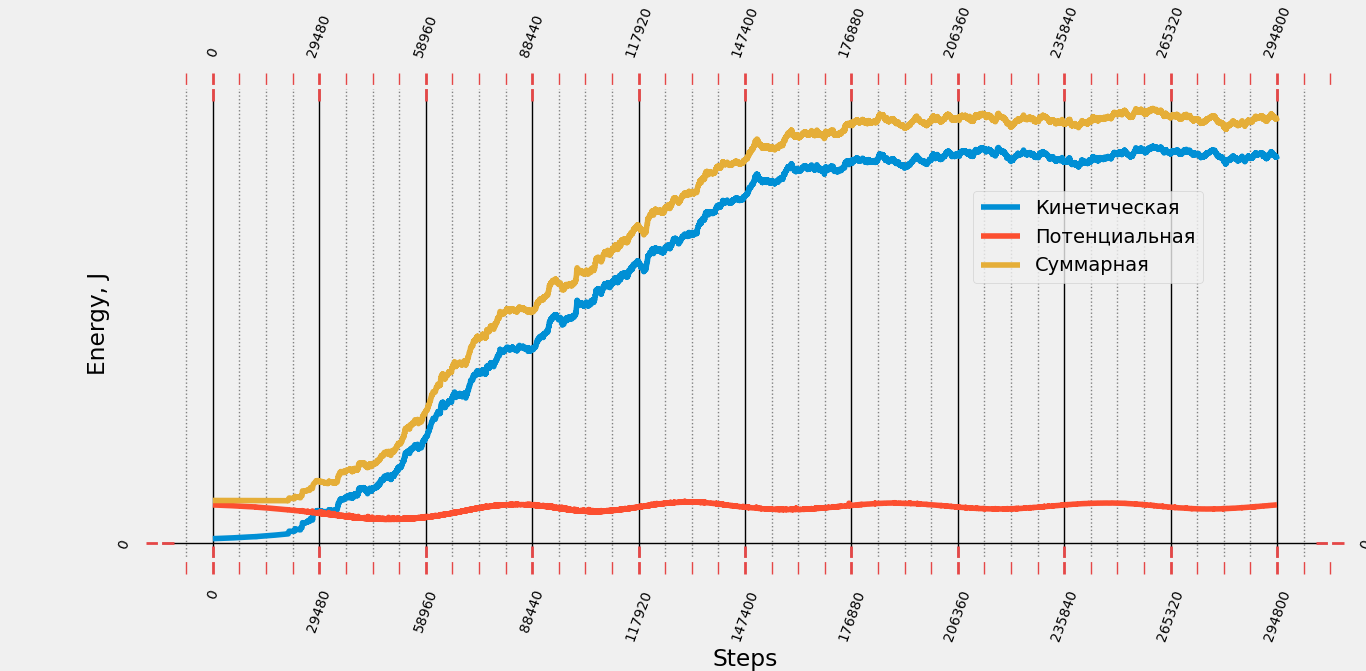
\includegraphics[width=0.5\textwidth]{kritic_energy} 
	\caption{График изменения энергии во времени при при превышении критической частоты}
	\label{pic:kritic_energy}
\end{figure} 


\newpage

\section{Заключение}

В представленной работе изучен метод дискретных элементов, а также была разработана математическая модель динамики частиц дроби в шаровой рудоразмольной мельнице.
В качестве примера применимости и работоспособности данной математической модели представлено сравнение с изученной моделью шаровой мельницы.
Разработанная модель позволяет исследовать режимы работы рудоразмольной мельницы.

\newpage

\renewcommand{\refname}{Список литературы}
\begin{thebibliography}{99}
\addcontentsline{toc}{section}{\refname}
\bibitem{cundall} Cundall P. A., Strack O. D. L. A discrete numerical model for granular assemblies //geotechnique. – 1979. – Т. 29. – №. 1. – С. 47-65.
\bibitem{friction_calibration} Syed Z., Tekeste M., White D. A coupled sliding and rolling friction model for DEM calibration //Journal of Terramechanics. – 2017. – Т. 72. – С. 9-20.
\bibitem{aglomerath} Караваев А. С., Копысов С. П., Сармакеева А. С. Моделирование динамики произвольных тел методом дискретных элементов //Вестник Удмуртского университета. Математика. Механика. Компьютерные науки. – 2015. – Т. 25. – №. 4. – С. 473-482.
\bibitem{mill_book} Андреев С. Е., Перов В. А., Зверевич В. В. Дробление, измельчение и грохочение полезных ископаемых. – Недра, 1980. – С. 415.
\end{thebibliography}


\end{document}